% \documentclass[aspectratio=169,notes]{beamer}
\documentclass[aspectratio=169]{beamer}
\usetheme[faculty=phil]{fibeamer}
\usepackage{polyglossia}
\setmainlanguage{english} %% main locale instead of `english`, you
%% can typeset the presentation in either Czech or Slovak,
%% respectively.
\setotherlanguages{russian} %% The additional keys allow
%%
%%   \begin{otherlanguage}{czech}   ... \end{otherlanguage}
%%   \begin{otherlanguage}{slovak}  ... \end{otherlanguage}
%%
%% These macros specify information about the presentation
\title[AGLA1]{Analytical Geometry and Linear Algebra I, Lab 12} %% that will be typeset on the
\subtitle{Test 2
\\ Polar coordinates   \\ \  
         } %% title page.
\author{Oleg Bulichev}
%% These additional packages are used within the document:
\usepackage{ragged2e}  % `\justifying` text
\usepackage{booktabs}  % Tables
\usepackage{tabularx}
\usepackage{tikz}      % Diagrams
\usetikzlibrary{calc, shapes, backgrounds}
\usepackage{amsmath, amssymb}
\usepackage{url}       % `\url`s
\usepackage{listings}  % Code listings
% \usepackage{subfigure}
\usepackage{floatrow}
\usepackage{subcaption}
\usepackage{mathtools}
\usepackage{todonotes}
\usepackage{fontspec}
\usepackage{multicol}
\usepackage{pdfpages}
\usepackage{wrapfig}
\usepackage{animate}
\usepackage{booktabs}
\usepackage{multirow}

\graphicspath{{resources/}}
\frenchspacing

\setbeamertemplate{caption}[numbered]
\usetikzlibrary{graphs}

% \usepackage[backend=biber,style=ieee,autocite=footnote]{biblatex}
% \addbibresource{biblio.bib}
% \DefineBibliographyStrings{english}{%
%   bibliography = {References},}

\newcommand{\oleg}[2][] {\todo[color=red, #1] {OLEG:\\ #2}}
\newcommand{\fbckg}[1]{\usebackgroundtemplate{\includegraphics[width=\paperwidth]{#1}}}%frame background

\usepackage[framemethod=TikZ]{mdframed}
\newcommand{\dbox}[1]{
\begin{mdframed}[roundcorner=3pt, backgroundcolor=yellow, linewidth=0]
\vspace{1mm}
{#1}
\vspace{1mm}
\end{mdframed}
}

\begin{document}
\setlength{\abovedisplayskip}{0pt}
\setlength{\belowdisplayskip}{0pt}
\setlength{\abovedisplayshortskip}{0pt}
\setlength{\belowdisplayshortskip}{0pt}

\fbckg{fibeamer/figs/title_page.png}
\frame[c]{\setcounter{framenumber}{0}
    \usebeamerfont{title}%
    \usebeamercolor[fg]{title}%
    \begin{minipage}[b][6.5\baselineskip][b]{\textwidth}%
        \textcolor{black}{\raggedright\inserttitle}
    \end{minipage}
    % \vskip-1.5\baselineskip

    \usebeamerfont{subtitle}%
    \usebeamercolor[fg]{framesubtitle}%
    \begin{minipage}[b][3\baselineskip][b]{\textwidth}
        \raggedright%
        \insertsubtitle%
    \end{minipage}
    \vskip.25\baselineskip
}
%   \frame[c]{\maketitle}

\fbckg{fibeamer/figs/common.png}

\note{\scriptsize \begin{itemize}
    \item Решения к ответам лежат в отдельной папке
\end{itemize}}


\begin{frame}[t]{Task 1, Var 1}
    \framesubtitle{}
    Find the equations of directrices and coordinates of focus (or foci) of the following curves:
    \begin{enumerate}
    \item  $x^2-2x+y=0$
    % \item $x+y-x^2+2xy-y^2=0$
    \end{enumerate}  \medskip
    
    \uncover<2->{
        \alert{\Large Algorithm}
        \begin{enumerate}
            \item Transform to canonical form (don't forget to change the variables, canonical form is a form, where is nothing near to $x$ and $y$ variables)
            \item Find parameters and coordinate dependent stuff in a new basis
            \item Represent $x'',\ y''$ respect to $x,\ y$ variables and substitute it in equations from previous step.
            \item Highlight answers.
        \end{enumerate}
    }
\end{frame}

\begin{frame}[t]{Task 2, Var 1}
    \framesubtitle{}
    Find the canonical equation of an ellipse (major axis is horizontal), if it is known that the eccentricity equals $0.5$ and the distance from its focus to the nearest vertex is 2.  \medskip
    
    \uncover<2->{
        \alert{\Large Algorithm}
        \begin{enumerate}
            \item Refresh the properties of each parameter by the cheat sheet.
            \item Draw a picture
            \item Based on it, find some parameters
            \item Find other parameters, knowing other stuff
        \end{enumerate}
    }
\end{frame}

\begin{frame}[t]{Task 3, Var 1}
    \framesubtitle{}
    Find the equations of the tangent and normal lines to the curve defined by the equation $x^2 - xy - y^2 + x + y = 0$ at the point with coordinates $(0.6,1.2)$ \medskip

    \uncover<2->{
        \alert{\Large Algorithm}
        \begin{enumerate}
            \item Task looks similar to lab 9, task 2. Or lab 10, task 5.
            \item Take a derivative $\frac{d y}{d x}$ --- slope ($k$).
            \item Knowing slope and the concrete coordinate, find $b$. Obtain needed equation.
            \item Either knowing the property $k_t k_n = -1$, find normal line. Or using the knowledge $A,\ B$ in general form is a normal vector.
        \end{enumerate}
    }
\end{frame}

\begin{frame}[t]{Task 4, Var 1}
    \framesubtitle{}
    \only<1>{
    In a triangle $ABC$ have vertices with coordinates $A(2,0); B(-1,2), C(-1,-2)$. 

    \begin{enumerate}
    
    \item Find the transform that maps each vertex of the triangle to the middle point of the opposite side. 
    
    \item Find the fixed point of the transform.
    
    \item How the area of the transformed triangle relates to the area of the triangle $ABC$.
    \end{enumerate}
    }
    \only<2>{
        \alert{\Large Algorithm}
        \begin{enumerate}
            \item (1) Draw a figure.
            \item For finding affine transformation, we should have 6 equations, hence $\rightarrow$ a mapping between $3$ points. Find such points by the figure.
            \item Solve $\underbrace{P_{mid}}_{[\vec{K}\vec{M}\vec{N}]}\underbrace{inv({P_{ver}})}_{[\vec{A}\vec{B}\vec{C}]} = H$. Don't forget to add $1$ in last column of each vector.
            \item (2) (Lab 12, task 1) $H\begin{bmatrix}x_{fix}\\y_{fix}\end{bmatrix}=\begin{bmatrix}x_{fix}\\y_{fix}\end{bmatrix}$. Find $x_{fix},\ y_{fix}$
            \item (3) Find determinant.
        \end{enumerate}
    }
\end{frame}

\begin{frame}[t]{Polar coordinates}
\framesubtitle{Straight Line}
\footnotesize
\begin{columns}[T,onlytextwidth]
    \begin{column}{0.49\textwidth}
        \vspace{-0.8cm}
        \begin{align}
            \label{eqn:p2c}
            \left\{\begin{matrix*}[l]
            x = r \cos(\phi)\\ 
            y = r \sin(\phi)
            \end{matrix*}\right. ,\ \text{where } \\
                r = \sqrt{x^2+y^2};
        \end{align}
    The general equation in polar coordinates ((\ref{eqn:p2c}) to $Ax+By+C=0$).
    \begin{align}
        \label{eqn:str_l}
        A\cos(\phi)+B\sin(\phi) + \frac{C}{r}=0
    \end{align}
    Eqn. of the line joining the 2 points:
    \begin{align*}
        \dfrac{1}{r}\sin(\phi_2-\phi_1)=\dfrac{1}{r_1}\sin({\phi_2-\phi}) + \dfrac{1}{r_2}\sin({\phi-\phi_1})
    \end{align*}
    \end{column}
    \begin{column}{0.49\textwidth}
        \vspace{-0.8cm}
        \begin{figure}[H]
            \centering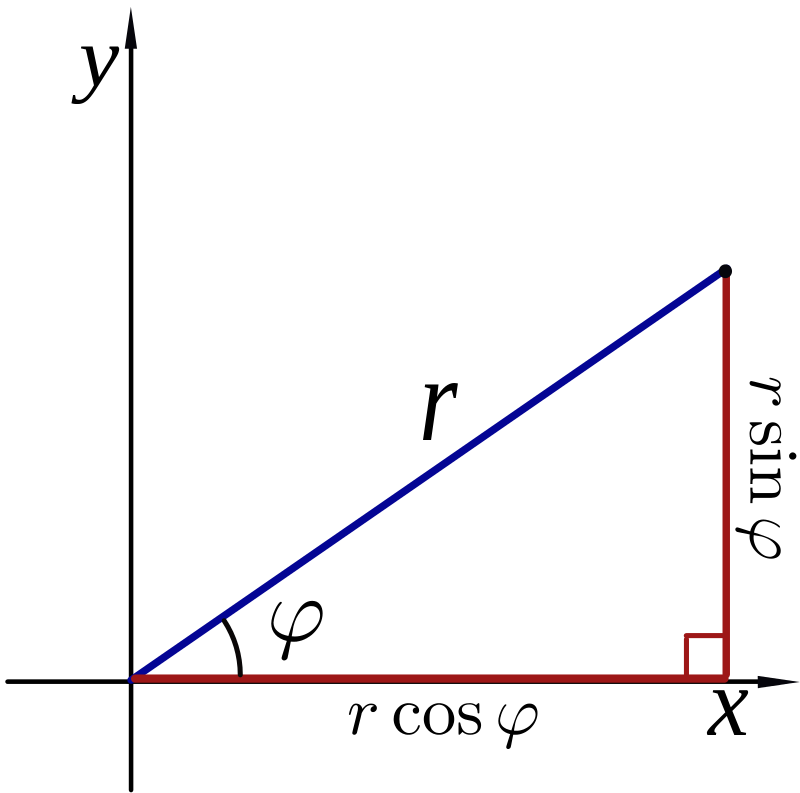
\includegraphics[height=2.8cm,width=1\textwidth,keepaspectratio]{polar_to_cart.png}
            % \caption{caption_name}
            \label{fig:polar_to_cart.png}
        \end{figure}
        \vspace{-0.5cm}
        Polar equation of the straight line perpendicular to (\ref{eqn:str_l})
        \begin{align*}
            A\cos(\phi+\frac{\pi}{2}) + B\sin(\phi+\frac{\pi}{2})=-k\frac{C}{r}
        \end{align*}
        Polar equation of the straight line parallel to (\ref{eqn:str_l}):
        \begin{align*}
            A\cos(\phi) + B\sin(\phi)=-k\frac{C}{r}
        \end{align*}
    \end{column}
\end{columns}
\end{frame}

\begin{frame}[t]{Task 1}
    \framesubtitle{}
    \only<1>{
        Find the equation of the line joining the points $\begin{bmatrix} 2 \\ \dfrac{\pi}{3} \end{bmatrix}$ and $\begin{bmatrix} 3 \\ \dfrac{\pi}{6} \end{bmatrix}$. It should deduce that this line also passes through the point $\begin{bmatrix} \dfrac{6}{3\sqrt{3}-2} \\ \dfrac{\pi}{2} \end{bmatrix}$.}
    \only<2>{
        \alert{\Large Answer}
        \begin{figure}[H]
            \centering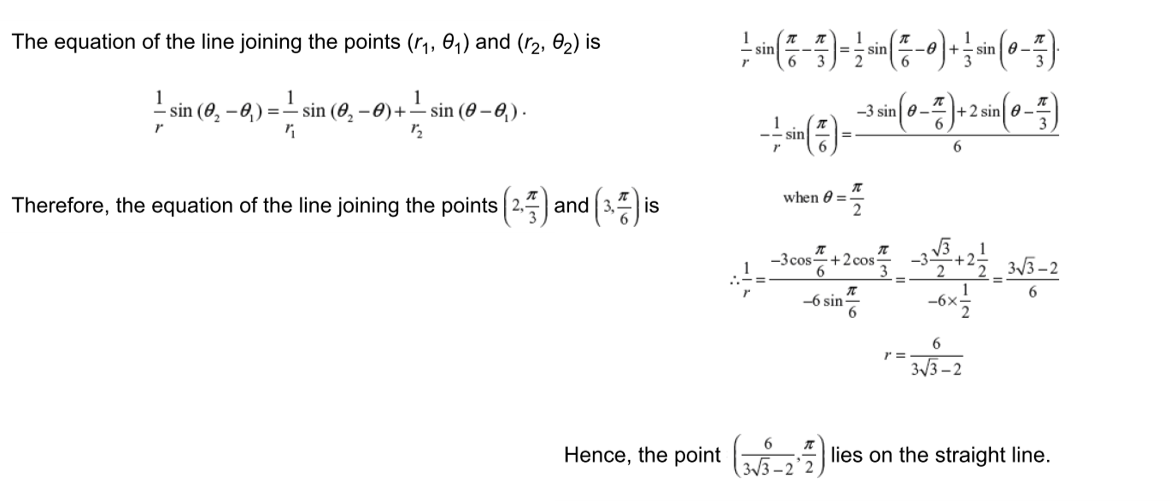
\includegraphics[height=5.5cm,width=1\textwidth,keepaspectratio]{1ans.png}
            % \caption{caption_name}
            \label{fig:1ans.png}
        \end{figure}
    }
\end{frame}

\begin{frame}[t]{Task 2}
    \framesubtitle{}
    \only<1>{
        Find the equation of the line perpendicular to $\dfrac{l}{r}=\cos(\theta-\alpha)+e\ \cos(\theta) $ and passing through the point $\begin{bmatrix} r_1 \\ \theta_1\end{bmatrix}$.}
    \only<2>{
        \alert{\Large Answer} \medskip

        $\dfrac{r_1 \sin(\theta_1 - \alpha) + e\ \sin(\theta_1)}{r}= \sin(\theta - \alpha) + e\ \sin(\theta)$
    }
\end{frame}

\begin{frame}[t]{Task 3}
    \framesubtitle{}
    \only<1>{
        Show that the feet of the perpendiculars from the origin on the sides of the triangle formed by the points with vectorial angles $\alpha,\ \beta,\ \gamma$ and which lie on the circle $r = 2a \cos(\theta)$ lie on the straight line $2a\ \cos(\alpha) \cos(\beta) \cos (\gamma) = r\ \cos(\pi - \alpha - \beta - \gamma)$.}
    \only<2>{
        \alert{\Large Answer}
        \begin{figure}[H]
            \centering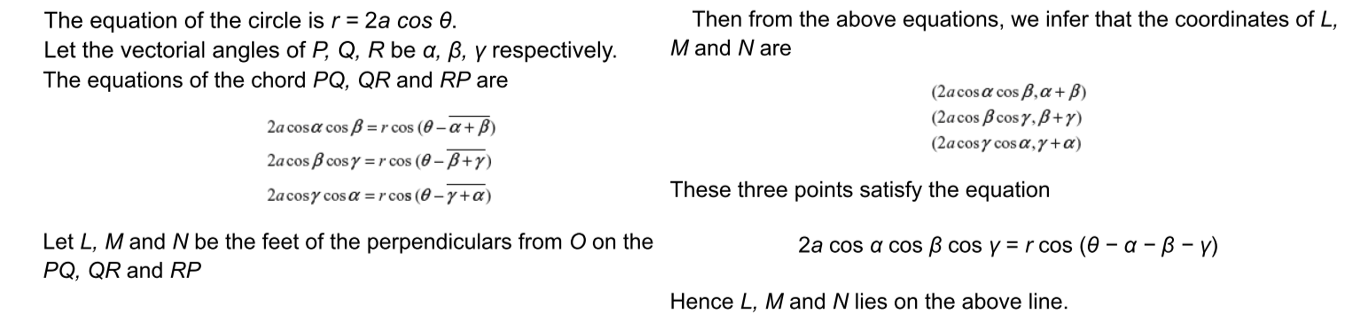
\includegraphics[height=5.5cm,width=1\textwidth,keepaspectratio]{3ans.png}
            % \caption{caption_name}
            \label{fig:3ans.png}
        \end{figure}
    }
\end{frame}

\begin{frame}[t]{Polar coordinates}
\framesubtitle{Conic Sections}
\footnotesize
    \begin{columns}[T,onlytextwidth]
        \begin{column}{0.49\textwidth}
            Equation of all types of conic section curves, when a conic is inclined at an angle $\alpha$ (if not inclined $\rightarrow \alpha=0$)
            \begin{align*}
                \frac{l}{r}=1+ecc\cos({\theta}-\alpha), \text{ where $l$ is semi-latus rectum}
            \end{align*}
            Polar equation of the directrix:
            \begin{align*}
                \frac{l}{r}=ecc\cos({\theta})
            \end{align*}
            Equation of tangent is given as
            \begin{align*}
                1+ ecc\cos({\theta}) + \cos(\theta-\alpha)=\frac{l}{r}
            \end{align*}
        \end{column}
        \begin{column}{0.49\textwidth}
            \begin{figure}[H]
                \centering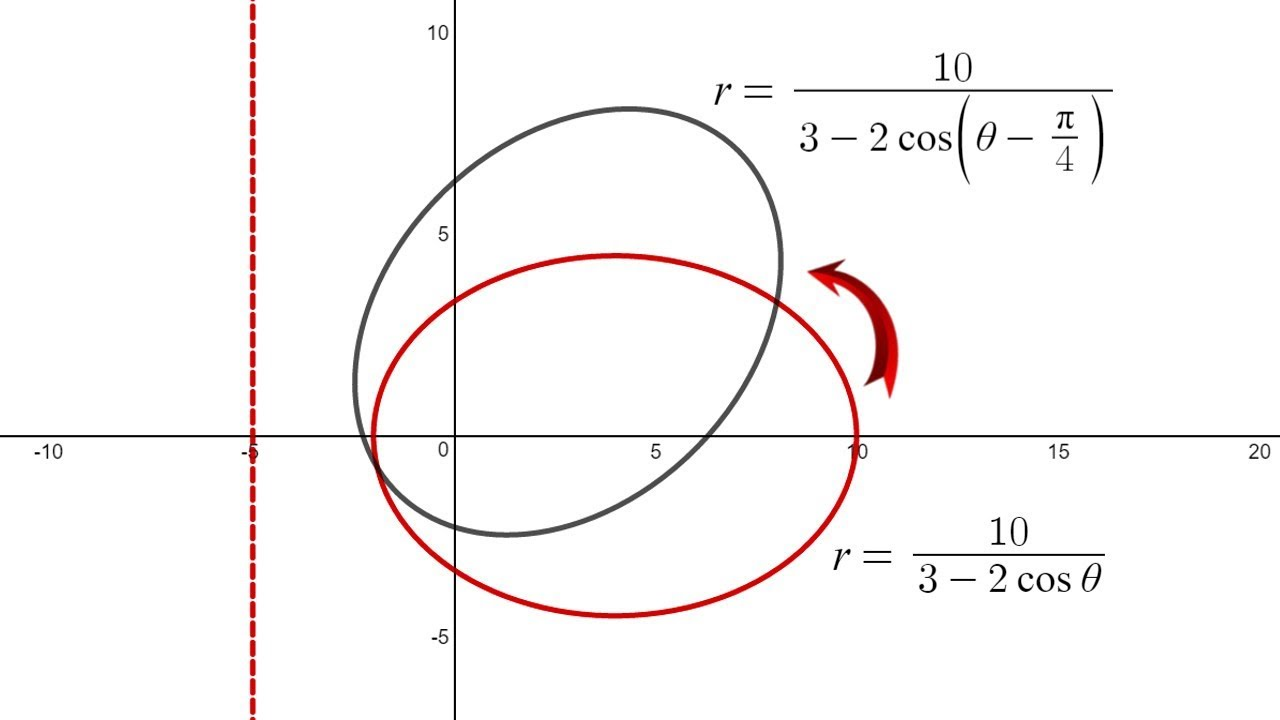
\includegraphics[height=6cm,width=1\textwidth,keepaspectratio]{conic_rot.jpg}
                % \caption{caption_name}
                \label{fig:conic_rot.jpg}
            \end{figure}
        \end{column}
    \end{columns}
\end{frame}

\begin{frame}[t]{Task 4}
    \framesubtitle{}
    \only<1>{
        A focal chord $SP$ of an ellipse is inclined at an angle $\alpha$ to the major axis. Prove that the perpendicular from the focus on the tangent at $P$ makes with the axis an angle $\arctan(\dfrac{\sin(\alpha)}{e+\cos(\alpha)})$}
    \only<2>{
        \alert{\Large Answer}
        \begin{figure}[H]
            \centering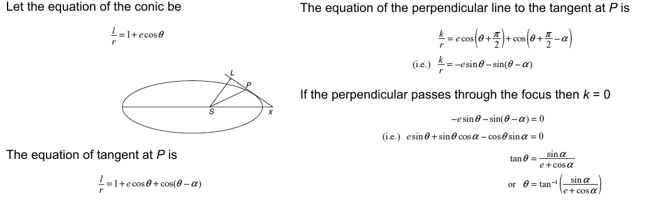
\includegraphics[height=5.5cm,width=1\textwidth,keepaspectratio]{4ans.png}
            % \caption{caption_name}
            \label{fig:4ans.png}
        \end{figure}
    }
\end{frame}


\begin{frame}[t]{Reference material}
    \Large
    \begin{itemize}
        \item \href{https://en.wikipedia.org/wiki/Polar_coordinate_system}{Polar coordinates (wiki)}
        \item \href{https://youtu.be/IAb98ZgSJNw}{Polar coordinates (video, eng)}
        \item \href{https://youtu.be/me3cBMfysZs}{Conics in Polar Coordinates: Rotation (video, eng)}
        \item \href{https://www.maths.tcd.ie/~stalker/22S1/MA22S1_Chapter_1.pdf}{Multivariable Calculus, chapter 1.2 Polar Coordinates (book, eng)}
    \end{itemize}
\end{frame}

\fbckg{fibeamer/figs/last_page.png}
\frame[plain]{}

\end{document}